\documentclass[xcolor=dvipsnames,table]{beamer}

\usepackage{latexsym}
\usepackage[utf8]{inputenc}
\usepackage[brazil]{babel}
\usepackage{amssymb}
\usepackage{amsmath}
\usepackage{stmaryrd}
\usepackage{fancybox}
\usepackage{datetime}
\usepackage[T1]{fontenc}
\usepackage{graphicx}
\usepackage{graphics}
\usepackage{url}
\usepackage{algorithmic}
\usepackage{algorithm}
\usepackage{acronym}
\usepackage{array}

\newtheorem{definicao}{Definio}
\newcommand{\tab}{\hspace*{2em}}

\mode<presentation>
{
  \definecolor{colortexto}{RGB}{0,0,0}
 
  \setbeamertemplate{background canvas}[vertical shading][ bottom=white!10,top=white!10]
  \setbeamercolor{normal text}{fg=colortexto} 

  \usetheme{Warsaw}
}

\title{Cortes} 

\author{
  Esdras Lins Bispo Jr. \\ \url{bispojr@ufg.br}
  } 
 \institute{
  Teoria de Grafos \\Bacharelado em Ciência da Computação}
\date{\textbf{05 de julho de 2017} }

\logo{
\includegraphics[width=1cm]{images/ufgJataiLogo.png}}

\begin{document}

	\begin{frame}
		\titlepage
	\end{frame}

	\AtBeginSection{
		\begin{frame}{Sumário}%[allowframebreaks]{Sumário}
    		\tableofcontents[currentsection]
    		%\tableofcontents[currentsection, hideothersubsections]
		\end{frame}
	}

	\begin{frame}{Plano de Aula}
		\tableofcontents
		%\tableofcontents[hideallsubsections]
	\end{frame}
    
   \begin{frame}{Pensamento}
   	\begin{columns}
   		\column{.4\textwidth}  		
   		\begin{center}
   			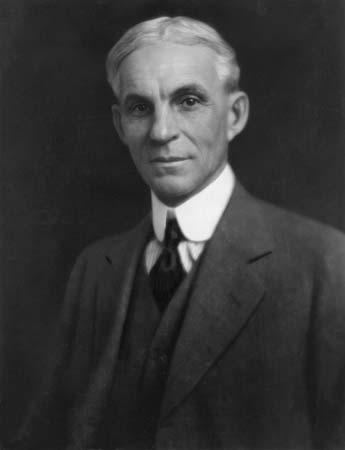
\includegraphics[width=.9\textwidth]{images/ford.jpg}
   		\end{center}
   		\column{.6\textwidth}  		
   		\begin{block}{Frase}
   			\begin{center}
   				{\large Corte sua própria lenha. Assim, ela aquecerá você duas vezes.}
   			\end{center}
   		\end{block}		  		
   		\begin{block}{Quem?}
   			\begin{center}
   				{\bf Henry Ford (1863 - 1947)} \\Empresário estadunidense.
   			\end{center}
   		\end{block}
   	\end{columns}
   \end{frame}
    
    \section{Revisão}
	\subsection{Grafos Conexos e Componentes}
	\begin{frame}{Grafos Conexos}
		\begin{block}{Definição}
			Um grafo é {\bf conexo} se, para qualquer par $\{v,w\}$ de seus vértices, existe um caminho com extremos $v$ e $w$.
		\end{block}
		\begin{block}{Subgrafo conexo maximal}
			Um subgrafo conexo $H$ de um grafo $G$ é maximal se $H$ não é subgrafo próprio de algum subgrafo conexo de $G$.
		\end{block}
		\begin{block}{Componente}
			Um {\bf componente} (ou {\bf componente conexo}) de um grafo $G$ é qualquer subgrafo conexo maximal de $G$.
		\end{block}
	\end{frame}
	
	\begin{frame}{Grafos Conexos}
		\begin{block}{Corolário 1}
			Cada vértice de um grafo pertence a um e um só componente.
		\end{block}
		\begin{block}{Corolário 2}
			Um grafo é conexo se e somente se tem um único componente.
		\end{block}
	\end{frame}

	\section{Cortes}
	\begin{frame}{Cortes}
		\begin{block}{Definição}
			\begin{itemize}
				\item Suponha que $X$ é um conjunto de vértices de um grafo $G$. \pause
				\item O {\bf corte} associado a $X$ (ou {\bf franja} de $X$) é o conjunto de todas as arestas que têm uma ponta em $X$ e outra em $V_G \setminus X$.
			\end{itemize}
		\end{block} \pause
		\begin{block}{Notação}
			O corte associado a $X$ será denotado por
			\begin{center}
				$\partial_G (X)$
			\end{center}
		\end{block} \pause
		\begin{alertblock}{Outros autores...}
			Alguns preferem escrever $\delta(X)$ ou $\nabla(X)$.
		\end{alertblock}
	\end{frame}
	
	\begin{frame}{Cortes}
		\begin{block}{Cortes triviais}
			\begin{itemize}
				\item $\partial( \emptyset )$; \pause
				\item $\partial( V_G )$.
			\end{itemize}
		\end{block} \pause
		\begin{block}{Corolário}
			$|\partial(\{v\})| = d(v)$
		\end{block} \pause
		\begin{block}{Grau de um conjunto}
			\begin{itemize}
				\item Diremos que $|\partial(X)|$ é o {\bf grau} de $X$; \pause
				\item Denotamos este número como se segue:
				\begin{center}
					$d(X) := |\partial(X)|$
				\end{center}
			\end{itemize}
		\end{block}
	\end{frame}
	
	\begin{frame}{Cortes}
		\begin{block}{Corte - Definição}
			Um {\bf corte} ({\it = cut = coboundary}) em um grafo $G$ é qualquer conjunto da forma $\partial(X)$, em que $X$ é um subconjunto de $V_G$.
		\end{block} \pause
		\begin{alertblock}{Cuidado}
			Um corte é um conjunto de arestas, não de vértices.
		\end{alertblock}
	\end{frame}
	
	\begin{frame}
		\titlepage
	\end{frame}
	
\end{document}